\documentclass[12pt]{article}
%Gumm{\color{blue}i}|065|=)
\usepackage{amsmath, amsfonts, amssymb}
\usepackage[margin=0.5in]{geometry}
\usepackage{xcolor}
\usepackage{graphicx}
\usepackage{amsmath}
\usepackage{hyperref}

\newcommand{\off}[1]{}
\DeclareMathSizes{20}{30}{20}{18}
\usepackage{tikz}


\title{Tune-Up: Cauchy Riemann Equations}
\date{}
\begin{document}

\sffamily

\maketitle

\noindent We learn in calculus class that $f(x) = x^2$ then $\frac{df}{dx} = 2x$. And this is a very special operation, since have a function and can turn it into another function. Let's remind ourselves how that one happened:
$$ \frac{df}{dx} = \lim_{\Delta x \to 0} \frac{f(x+\Delta x) - f(x) }{\Delta x} = \lim_{\Delta x \to 0}\frac{(x + \Delta x)^2 - x^2}{\Delta x} $$
Let's see if we can do anything about the expression in the limit:
$$ \frac{ \big(x^2 + 2x \, \Delta x + (\Delta x)^2 \big) - x^2 }{\Delta x} 
= \frac{ \Delta x \big(  2x + \Delta x \big) }{\Delta x} = 2x + \Delta x \to 2x + [0]$$
Notice the division works out perfectly.  And for this class of functions it always does. \\ \\
Let's draw the picture.  This is easy enough to draw with only \texttt{tikz}.\\ \\
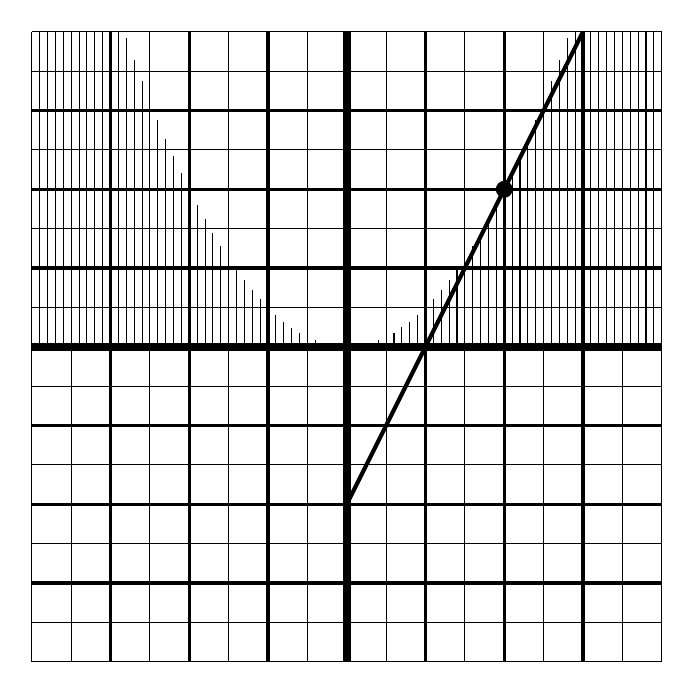
\begin{tikzpicture}[scale=1]
\draw[line width=3] (-4,0)--(4,0);
\draw[line width=3] (0,-4)--(0,4);

\foreach \a in {-4,-3.5,...,4}{
	\draw (\a,-4)--(\a,4);
	\draw (-4,\a)--(4,\a);
}

\foreach \a in {-3,...,3}{
	\draw[line width =1.25] (\a,-4)--(\a,4);
	\draw[line width =1.25] (-4,\a)--(4,\a);
}


\foreach \a in {-2.8,-2.7,...,2.9}{
	\draw (\a,0)--(\a,0.5*\a*\a);
}
\foreach \a in {-4,-3.9,...,-2.8}{
	\draw (\a,0)--(\a,4);
}

\foreach \a in {2.9,3,...,4}{
	\draw (\a,0)--(\a,4);
}

\draw[line width=1.5] (3,4)--(0,-2);

\draw[fill=black] (2,2) circle (0.1);


\end{tikzpicture} \\ 
Here we were able to \textit{parameterize} the curve well enough to draw, let's see if we're so lucky in future circumstances. \\ \\
In the mean time, let consider what happens when $\Delta x \neq 0$.  Let's say $0 < \Delta x = 0.1 \ll 1$.  Then let's take square:
$$  (1 + 0.1)^2 = 1.21 \text{ yet } (1+0.1)^2 \approx 1 + 2 \times 1 \times 0.1 = 1.2$$
We are off by less than 1\%.  So this is a pretty good most of the time.  We're going to be OK. \\ \\
In fact, Taylor's theorem says that we're almost always going to be OK, no matter what function we choose:
$$ f(x + \Delta x) \approx f(x) + \Delta x \cdot \frac{\Delta f}{\Delta x} + O(\Delta x^2) $$
Therefore line and parabola should do the job almost every single time.  Any further doubts require the \textbf{Mean Value Theorem}.

\newpage \noindent The complex analysis textbook begins the same way.  Let $f(z) = z^2$.  Then 
$$  f(z) = z^2 \text{ then } \frac{df}{dz} = \lim_{\Delta z \to 0} \frac{(z + \Delta z)^2 - z^2}{\Delta z} = 2z + O(\Delta z)$$
We even have a sort of guarantee of how far our line is.  Let's try to check and makes sure we understand what $|\Delta z| \to 0$ really means. \\ \\ 
$z^2 = (x + iy)^2 = (x^2 - y^2) + i(2xy)$. \\ \\
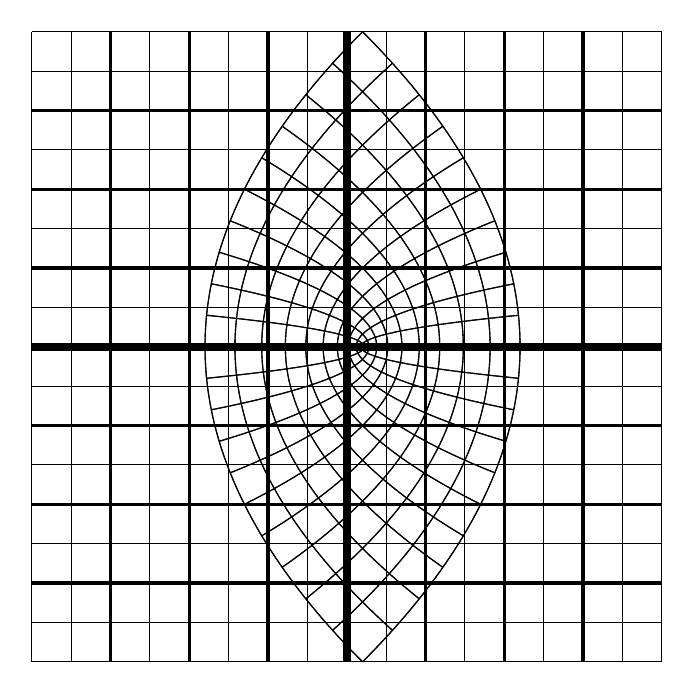
\begin{tikzpicture}

\begin{scope}

\draw[line width=3] (-4,0)--(4,0);
\draw[line width=3] (0,-4)--(0,4);

\foreach \a in {-4,-3.5,...,4}{
	\draw (\a,-4)--(\a,4);
	\draw (-4,\a)--(4,\a);
}

\foreach \a in {-3,...,3}{
	\draw[line width =1.25] (\a,-4)--(\a,4);
	\draw[line width =1.25] (-4,\a)--(4,\a);
}

\end{scope}

\begin{scope}[scale=0.02, xshift=10cm]
\foreach \a in {-10,-9,...,10}{
	\foreach \b in {-10,-9.9,...,10}{
		\draw (\a*\a - \b*\b ,2*\a*\b)--( {\a*\a-(\b+0.1)*(\b+0.1)} , {2*\a*(\b+0.1)});
	}
}

\foreach \a in {-10,-9.9,...,10}{
	\foreach \b in {-10,-9,...,10}{
		\draw (\a*\a - \b*\b ,2*\a*\b)--( {(\a+0.1)*(\a+0.1)-\b*\b} , {2*\b*(\a+0.1)});
	}
}
\end{scope}

\end{tikzpicture} \\ \\
Drawing this picture has cost a lot of computing time, and it still doesń t look quite right.  Perhaps I need to use an algorithm. 
\vfill
\begin{thebibliography}{} 
\item Vladimir Zorich \textbf{Mathematical Analysis I} (Universitext) Springer, 2015.
\end{thebibliography}

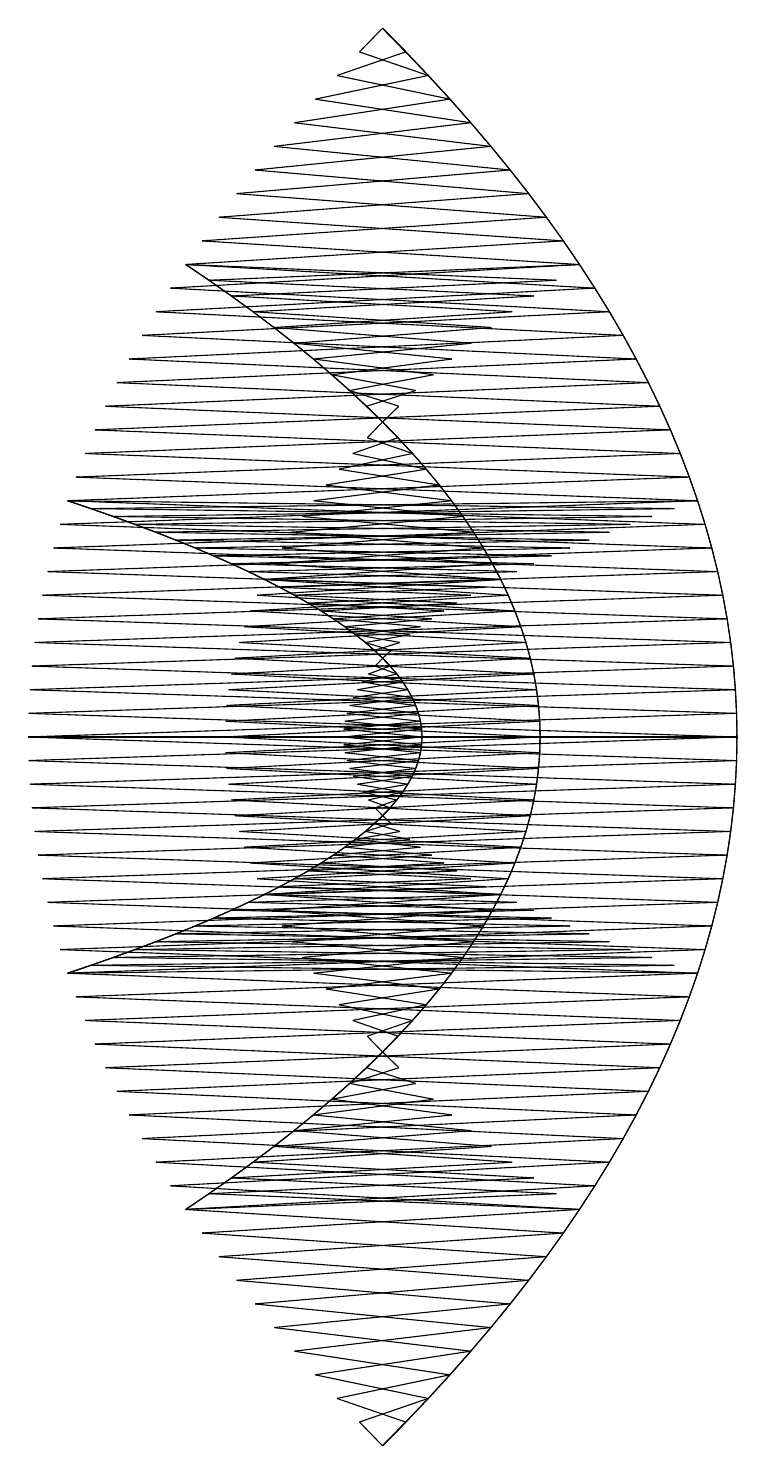
\begin{tikzpicture}[scale = 0.5]

\foreach \a in {-3,-2,...,3}{
	\foreach \b in {-3,-2.9,...,3}{
		%\draw (\a*\a - \b*\b, 2*{\a*\b} )--(0,0);
		\draw (\a*\a - \b*\b ,2*\a*\b)--( {\a*\a-(\b+0.1)*(\b+0.1)} , {2*\a*(\b+0.1)});
		\draw (\b*\b - \a*\a ,2*\a*\b)--( {\a*\a-(\b+0.1)*(\b+0.1)} , {2*\a*(\b+0.1)});
	}
}
\end{tikzpicture}
\end{document}